\begin{quote}\small\textbf{观课提示}\quad 观察小矩形累积以及误差方向，再把积分解释成端点变化。

\href{https://www.youtube.com/watch?v=rfG8ce4nNh0}{原课程视频}\quad\href{https://vitael04213.github.io/3blue1brown-notes/lessons/integration.html}{本节网页与媒体}\quad\href{https://vitael04213.github.io/3blue1brown-notes/lab.html\#integral}{参数实验}
\end{quote}
\begin{figure}[htbp]\centering
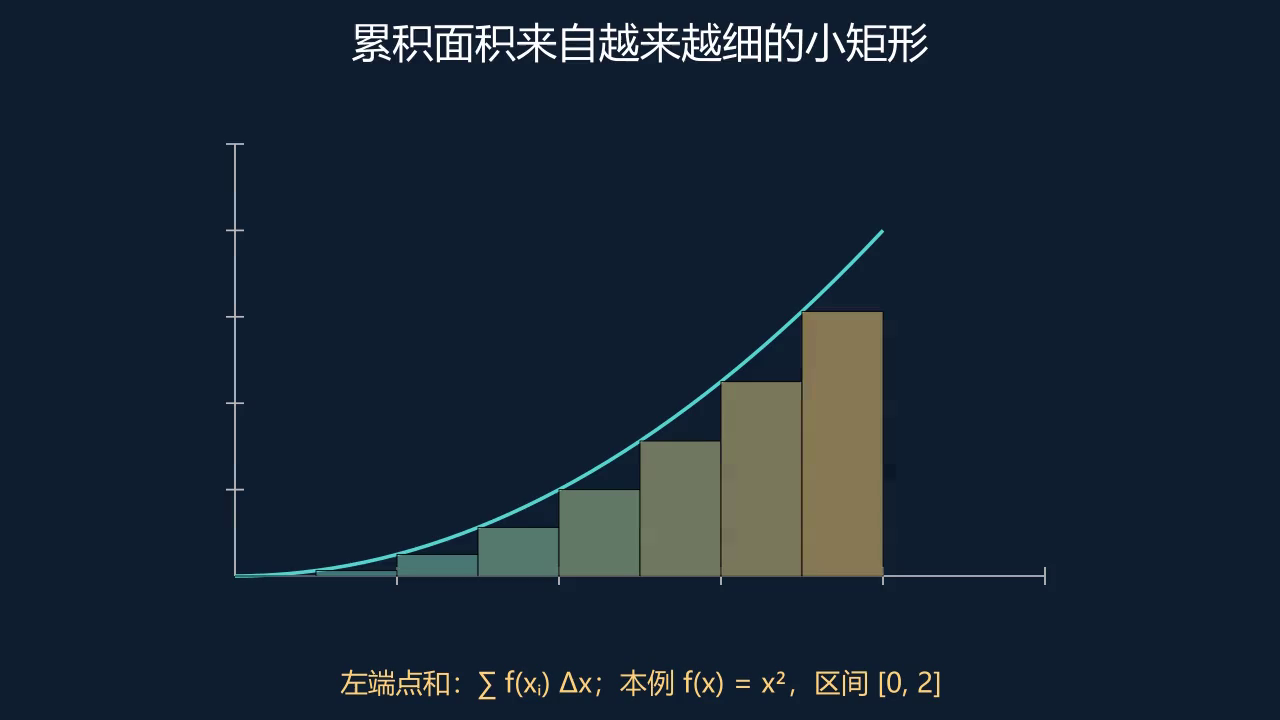
\includegraphics[width=0.98\linewidth]{figures/Integral.png}
\caption{平方函数的左端点矩形和。切分变细时，累积面积逐渐接近积分。本项目原创 Manim 动画关键帧；完整动画与操作入口见本节网页。}
\end{figure}
